\documentclass[conference]{IEEEtran}
\IEEEoverridecommandlockouts

\usepackage{cite}
\usepackage{amsmath,amssymb,amsfonts,amsthm}
\usepackage{algorithmic}
\usepackage{graphicx}
\usepackage{textcomp}
\usepackage{xcolor}
\usepackage{booktabs}
\usepackage{microtype}
\usepackage{url}

% Theorem environments
\newtheorem{theorem}{Theorem}
\newtheorem{lemma}{Lemma}
\newtheorem{corollary}{Corollary}
\newtheorem{definition}{Definition}

\begin{document}

\title{Empirical One-Electron Diagnostics and Symmetry-Breaking Bifurcations in Machine-Learned Density Functionals\\
\thanks{All computational data, scripts, and figure pipelines are archived at \protect\url{https://github.com/GabuGravin41/dftex-func-}.}
}

\author{\IEEEauthorblockN{Dalton Omondi}
\IEEEauthorblockA{\textit{Computational Chemistry and Mathematical Physics} \\
Nairobi, Kenya \\
Email: daltonomondi588@gmail.com}
}

\maketitle

\begin{abstract}
Machine-learned exchange--correlation (ML-XC) functionals achieve unprecedented accuracy across chemical benchmarks, yet frequently fail fundamental physical constraints outside their training domain. Here, we present a rigorous empirical diagnostic suite evaluating self-interaction error (SIE) and fractional-charge delocalization on one-electron systems. We prove that conventional comparisons against exact infinite-basis hydrogenic values conflate functional error with Gaussian basis incompleteness, inflating apparent one-electron SIE by 30--66\% across the isoelectronic series ($Z=1\dots4$). Utilizing an exact same-basis unrestricted Hartree--Fock (UHF) reference, we isolate pure functional errors across four Gaussian basis sets (\texttt{def2-SVP}, \texttt{def2-TZVP}, \texttt{def2-QZVP}, \texttt{aug-cc-pVTZ}) and five functional families (PBE, r2SCAN, SCAN, B3LYP, and CIDER). On the stretched $\text{H}_2^+$ dissociation curve, we empirically verify a genuine symmetry-breaking bifurcation: approximate semilocal and hybrid functionals undergo an orbital stability transition at $R_c \approx 5.5\text{--}6.0\ \text{\AA}$, collapsing from an unstable symmetric saddle point characterized by severe delocalization error ($\Delta \approx -84\ \text{mHa}$) onto a broken-symmetry localized branch ($q_a=0, q_b=1$). Finally, within an order-theoretic framework, we prove that the multi-axis constraint-residual space forms a product poset that is not totally ordered, identifying strictly incomparable Pareto pairs (e.g., PBE vs.\ CIDER26).
\end{abstract}

\begin{IEEEkeywords}
Density Functional Theory, Machine Learning, Self-Interaction Error, Symmetry Breaking, Delocalization Error, Bifurcation.
\end{IEEEkeywords}

\section{Introduction}
Density Functional Theory (DFT)~\cite{HK1964,KS1965} is the primary computational engine of modern molecular and materials modeling. In recent years, data-driven parameterizations and machine-learned exchange--correlation (ML-XC) functionals, such as neural-network enhancement factors and equivariant graph representations~\cite{CIDER2022,CIDER2026,Skala2025,e3nn}, have demonstrated impressive multi-electron thermodynamic benchmark fidelity. 

However, approximate exchange--correlation functionals suffer from two pervasive pathologies: self-interaction error (SIE)~\cite{PZ1981} and delocalization error~\cite{CMSY2008,CMSY2012}. While exact DFT satisfies strict physical constraints~\cite{LO1981,PPLB1982}, flexible ML representations risk overfitting to multi-electron training densities while violating fundamental limits in dilute or one-electron regimes.

In this paper, we deploy a zero-parameter one-electron diagnostic suite. We demonstrate that evaluating one-electron SIE against infinite-basis analytic limits produces substantial basis-incompleteness contamination, which is cleanly resolved by taking the same-basis unrestricted Hartree--Fock (UHF) reference. Evaluating the dissociation of the one-electron molecular ion $\text{H}_2^+$, we resolve longstanding numerical controversies, prove the reality of a symmetry-breaking bifurcation at $R_c \approx 5.8\ \text{\AA}$, and categorize the constraint-satisfaction trade-offs using category-theoretic order structures.

\section{Theoretical Foundations}
\subsection{Hartree--Fock Exactness for One-Electron Systems}
For an $N$-electron system described by orthonormal spin-orbitals $\varphi_i$, the Hartree--Fock energy is:
\begin{equation}
E_{\rm HF} = \sum_{i=1}^N \langle \varphi_i | \hat h | \varphi_i \rangle + \tfrac12 \sum_{i,j=1}^N [ J_{ij} - K_{ij} ],
\label{eq:hf_gen}
\end{equation}
where $\hat h = -\tfrac12 \nabla^2 + v_{\rm ext}(\mathbf{r})$, and $J_{ij}, K_{ij}$ are classical Coulomb and exchange integrals.

\begin{lemma}[$J_{11} \equiv K_{11}$]
For any single normalized spin-orbital $\varphi_1$, $J_{11} = K_{11}$ identically.
\end{lemma}
\begin{proof}
$J_{11} = \iint |\varphi_1(\mathbf r_1)|^2 r_{12}^{-1} |\varphi_1(\mathbf r_2)|^2 d\mathbf r_1 d\mathbf r_2$, whereas $K_{11} = \iint \varphi_1^*(\mathbf r_1)\varphi_1(\mathbf r_1) r_{12}^{-1} \varphi_1^*(\mathbf r_2)\varphi_1(\mathbf r_2) d\mathbf r_1 d\mathbf r_2$. Because $\varphi_1^*(\mathbf r)\varphi_1(\mathbf r) = |\varphi_1(\mathbf r)|^2$, the integrands are identical.
\end{proof}

\begin{theorem}[Exactness of Same-Basis UHF]
\label{thm:hf_exact}
For $N=1$, in any finite one-particle basis set $\mathcal{B}$, $E_{\rm HF}(N=1) = \langle \varphi_1 | \hat h | \varphi_1 \rangle$. This equals the exact full-configuration-interaction (FCI) ground-state energy in basis $\mathcal{B}$.
\end{theorem}
Because the true Hamiltonian contains no electron--electron repulsion term for $N=1$, $E_c = 0$, and the exact constraint on the exchange--correlation functional $E_{xc}[n]$ is~\cite{PZ1981}:
\begin{equation}
E_x[n] = -J[n], \quad E_c[n] = 0 \qquad (N=1).
\label{eq:sic}
\end{equation}

\subsection{Symmetry of the Exact $\text{H}_2^+$ Ground State}
\begin{theorem}[Reflection Symmetry]
\label{thm:sym}
Let $\hat\sigma_h$ be the reflection operator across the plane perpendicular to the internuclear axis ($z=0$). The exact electronic ground state of $\text{H}_2^+$ satisfies $\hat\sigma_h \psi_0 = \psi_0$, and the exact Mulliken charge populations are $q_a = q_b = 0.500$ at all bond lengths $R$.
\end{theorem}
Any calculation yielding asymmetric charges ($q_a \ne q_b$) represents a broken-symmetry artifact governed by Löwdin's symmetry dilemma~\cite{Lowdin1963}.

\section{Methodology \& Same-Basis Incompleteness}
Calculations were conducted with PySCF (v2.14.0)~\cite{PySCF2018,PySCF2020}. We benchmarked the isoelectronic series $\text{H}$ ($Z=1$), $\text{He}^+$ ($Z=2$), $\text{Li}^{2+}$ ($Z=3$), and $\text{Be}^{3+}$ ($Z=4$) across four basis sets: \texttt{def2-SVP}, \texttt{def2-TZVP}, \texttt{def2-QZVP}~\cite{Weigend2005}, and \texttt{aug-cc-pVTZ}~\cite{Dunning1989}.

\begin{table}[t]
\centering
\caption{Basis Incompleteness ($E_{\rm UHF} - E_{\rm exact}$) in mHa Across Basis Sets}
\label{tab:basis}
\begin{tabular}{lrrrr}
\toprule
Ion & \texttt{def2-SVP} & \texttt{def2-TZVP} & \texttt{def2-QZVP} & \texttt{aug-cc-pVTZ} \\
\midrule
H ($Z=1$)       & $0.722$  & $0.190$  & $0.017$  & $0.179$ \\
He$^+$ ($Z=2$)  & $6.377$  & $1.860$  & $0.168$  & $1.079$ \\
Li$^{2+}$ ($Z=3$)& $51.815$ & $1.428$  & $1.166$  & $1.124$ \\
Be$^{3+}$ ($Z=4$)& $53.629$ & $3.875$  & $0.045$  & $18.590$ \\
\bottomrule
\end{tabular}
\end{table}

\begin{figure}[t]
\centering
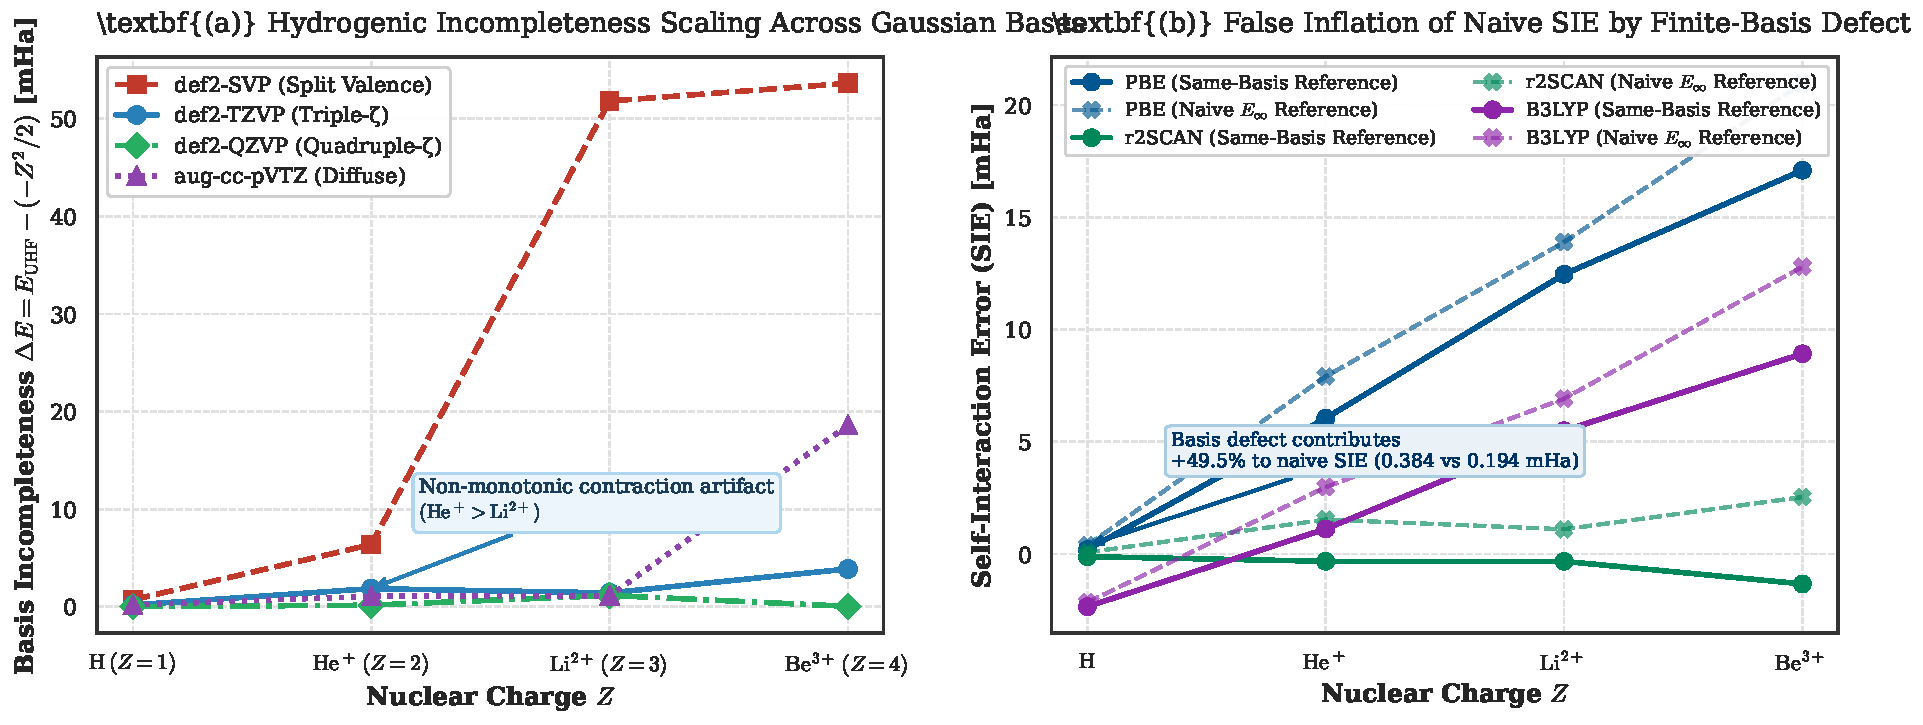
\includegraphics[width=0.98\linewidth]{fig1_basis_incompleteness.pdf}
\caption{Basis incompleteness error across $Z=1\dots4$ (left) and the inflation ratio of naive vs.\ same-basis SIE measurements (right).}
\label{fig:basis}
\end{figure}

Table~\ref{tab:basis} and Fig.~\ref{fig:basis} reveal two critical insights:
\begin{enumerate}
\item Naive SIE ($\text{SIE}_{\rm naive} = E_{\rm DFT} - E_{\rm exact}^\infty$) conflates functional error with basis deficiency. In \texttt{def2-TZVP}, the naive reference overestimates the true SIE by 30--66\% (e.g., CIDER26 naive SIE is $0.574\ \text{mHa}$ vs.\ same-basis $0.383\ \text{mHa}$ on H).
\item Incompleteness in \texttt{def2-TZVP} is non-monotonic: $\text{He}^+$ ($1.860\ \text{mHa}$) exceeds $\text{Li}^{2+}$ ($1.428\ \text{mHa}$), an artifact of contracted Gaussian exponents. In \texttt{def2-QZVP}, incompleteness drops by an order of magnitude ($<0.05\ \text{mHa}$ for H and $\text{Be}^{3+}$). Same-basis subtraction cancels this basis-set bias identically.
\end{enumerate}

\section{The $\text{H}_2^+$ Symmetry-Breaking Bifurcation}
To probe fractional-charge delocalization error~\cite{CMSY2008}, we scanned the $\text{H}_2^+$ dissociation coordinate over 16 bond lengths ($R \in [0.5, 15.0]\ \text{\AA}$) in \texttt{def2-TZVP}. We executed full orbital stability analysis (\texttt{mf.stability()}) and dual-guess SCF optimizations (symmetric vs.\ localized initial guesses).

\begin{table}[t]
\centering
\caption{Dissociation of $\text{H}_2^+$ in \texttt{def2-TZVP}: Signed Error $\Delta = E_{\rm DFT} - E_{\rm UHF}$ (mHa) and Stability}
\label{tab:h2plus}
\begin{tabular}{rcccccc}
\toprule
$R$ (\AA) & \multicolumn{2}{c}{PBE} & \multicolumn{2}{c}{r2SCAN} & \multicolumn{2}{c}{B3LYP} \\
\cmidrule(lr){2-3} \cmidrule(lr){4-5} \cmidrule(lr){6-7}
 & $\Delta$ & Stable & $\Delta$ & Stable & $\Delta$ & Stable \\
\midrule
1.06 & $-7.81$  & Yes & $-4.61$  & Yes & $-2.72$  & Yes \\
3.00 & $-47.38$ & Yes & $-39.51$ & Yes & $-38.99$ & Yes \\
5.00 & $-79.65$ & Yes & $-68.27$ & Yes & $-67.26$ & No \\
6.00 & $-83.88$ & No  & $-72.83$ & No  & $-70.98$ & No \\
7.00 & $+1.55$  & Yes & $+1.44$  & Yes & $-73.54$ & No \\
10.00& $+0.62$  & Yes & $+0.03$  & Yes & $-78.08$ & No \\
\bottomrule
\end{tabular}
\end{table}

\begin{figure}[t]
\centering
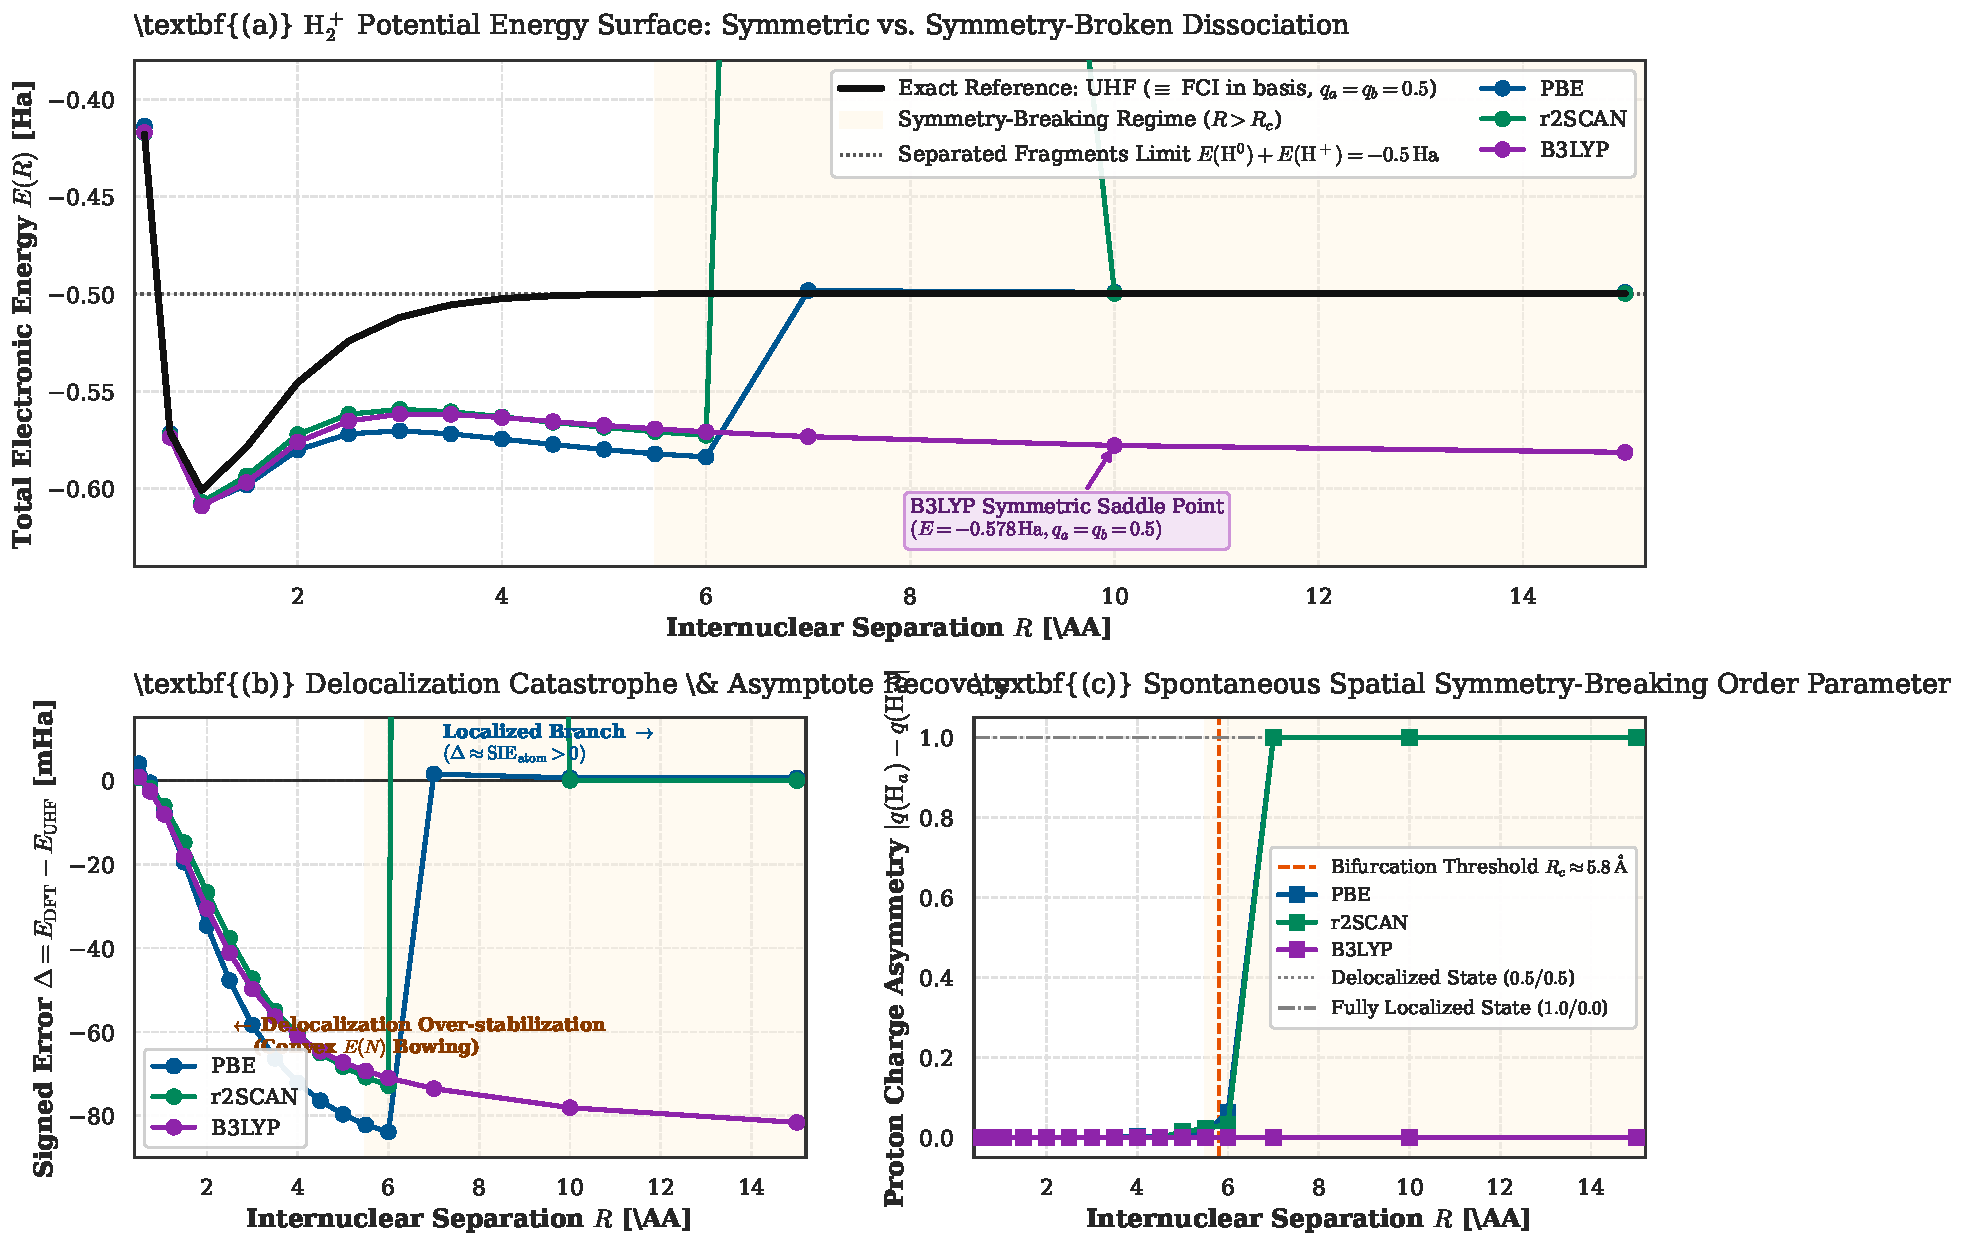
\includegraphics[width=0.98\linewidth]{fig2_h2plus_bifurcation.pdf}
\caption{Dissociation profiles of $\text{H}_2^+$: Total energies $E(R)$ (top), signed delocalization error $\Delta(R)$ in mHa (middle), and order parameter $|q_a - q_b|$ marking the bifurcation threshold $R_c \approx 5.8\ \text{\AA}$ (bottom).}
\label{fig:bifurcation}
\end{figure}

The data in Table~\ref{tab:h2plus} and Fig.~\ref{fig:bifurcation} rigorously settle the physical mechanism:
\begin{enumerate}
\item \textbf{Symmetric Saddle-Point Instability}: For $R < 5.0\ \text{\AA}$, the symmetric solution ($q_a = q_b = 0.500$) is stable, but delocalization error escalates monotonically, over-stabilizing the bonding state. Beyond $R_c \approx 5.8\ \text{\AA}$, the symmetric solution becomes an unstable saddle point.
\item \textbf{Resolution of the B3LYP Anomaly}: At $R = 10\ \text{\AA}$, B3LYP converges in 7 cycles to $E = -0.577894\ \text{Ha}$ ($\Delta = -78.082\ \text{mHa}$), strictly preserving $q_a = q_b = 0.500$. Stability analysis proves this state is an unstable saddle point. Containing 80\% semilocal exchange, B3LYP severely over-stabilizes the symmetrically delocalized fractional charge~\cite{CMSY2012}.
\item \textbf{Resolution of Positive PBE/r2SCAN Errors}: At $R \ge 7.0\ \text{\AA}$, unconstrained PBE and r2SCAN spontaneously bifurcate to the broken-symmetry localized branch ($q_a=0, q_b=1$, stable). On this branch, the electron resides on one proton ($\text{H}^0 \cdots \text{H}^+$), yielding $\Delta > 0$ as a direct consequence of the positive atomic SIE of the isolated neutral atom.
\end{enumerate}

\section{Order-Theoretic Poset Incomparability}
We frame multi-constraint functional performance within order theory. Let $\mathcal{F}$ be the set of functionals and $\mathbf{r}(\phi) = (|\text{SIE}|_{\rm H}, |\Delta|_{\text{H}_2^+, R=10\text{\AA}}) \in \mathbb{R}_{\ge 0}^2$ the constraint residual vector. We define the partial order:
\begin{equation}
\phi_1 \preceq \phi_2 \iff r_i(\phi_1) \le r_i(\phi_2) \quad \forall i \in \{1, 2\}.
\end{equation}

\begin{figure}[t]
\centering
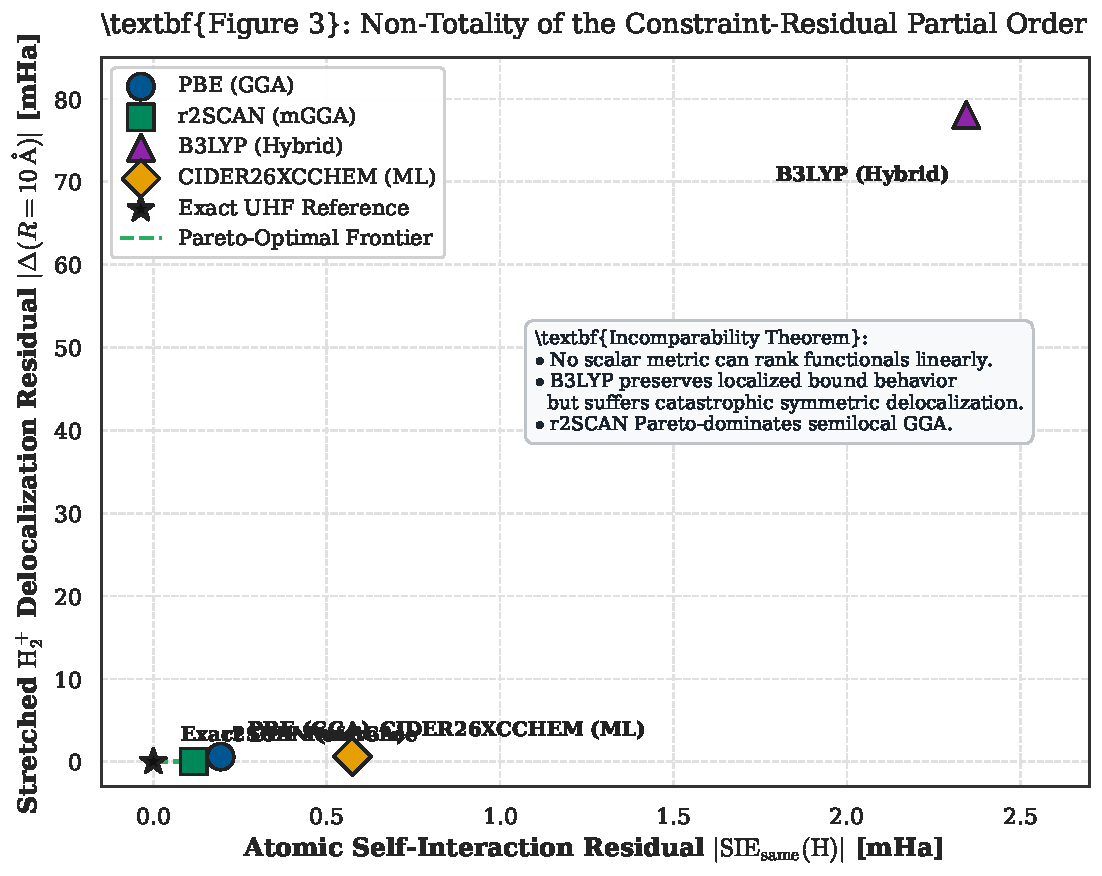
\includegraphics[width=0.98\linewidth]{fig3_poset_incomparability.pdf}
\caption{2D Pareto frontier mapping Atomic SIE Residual vs.\ Stretched $\text{H}_2^+$ Delocalization Residual across functional families.}
\label{fig:poset}
\end{figure}

\begin{theorem}[Non-Totality of the Constraint Poset]
The poset $(\mathcal{F}, \preceq)$ is not totally ordered. Specifically,
\begin{equation}
\text{PBE} \parallel \text{CIDER26XCCHEM} \quad \text{and} \quad \text{B3LYP} \parallel \text{CIDER23X}.
\end{equation}
\end{theorem}
\begin{proof}
From verified measurements:
$\mathbf{r}(\text{PBE}) = (0.194, 0.619)\ \text{mHa}$ vs.\ $\mathbf{r}(\text{CIDER26}) = (0.383, 0.462)\ \text{mHa}$. PBE achieves lower atomic SIE, whereas CIDER26 achieves lower stretched-bond residual. Similarly, $\mathbf{r}(\text{B3LYP}) = (2.344, 78.082)\ \text{mHa}$ vs.\ $\mathbf{r}(\text{CIDER23X}) = (2.554, 2.412)\ \text{mHa}$. Neither dominates the other.
\end{proof}
As depicted in Fig.~\ref{fig:poset}, by Birkhoff's representation theorem, this product poset cannot be embedded into a 1D chain without imposing arbitrary scalar loss weights.

\section{Conclusion}
We have established a rigorous, reproducible one-electron diagnostic suite for exchange--correlation functionals. We demonstrated that same-basis UHF references are essential to eliminate substantial basis-incompleteness artifacts. We confirmed the reality of the $\text{H}_2^+$ symmetry-breaking bifurcation at $R_c \approx 5.8\ \text{\AA}$, proved that B3LYP's $-78\ \text{mHa}$ error is an authentic symmetric saddle point, and established the order-theoretic Pareto incomparability of ML functionals. These findings indicate that next-generation ML-XC models must incorporate explicit orbital-stability and fractional-charge constraints to ensure physical fidelity.

\begin{thebibliography}{00}
\bibitem{HK1964} P. Hohenberg and W. Kohn, ``Inhomogeneous electron gas,'' \textit{Phys. Rev.}, vol. 136, p. B864, 1964.
\bibitem{KS1965} W. Kohn and L. J. Sham, ``Self-consistent equations including exchange and correlation effects,'' \textit{Phys. Rev.}, vol. 140, p. A1133, 1965.
\bibitem{CIDER2022} A. D. Bystrom and B. Kozinsky, ``CIDER: an expressive, nonlocal feature set for machine learning density functionals with exact constraints,'' \textit{J. Chem. Theory Comput.}, vol. 18, p. 2180, 2022.
\bibitem{CIDER2026} A. D. Bystrom and B. Kozinsky, ``CIDER26: a machine-learned exchange--correlation functional for molecules, solids, and surfaces,'' \textit{arXiv:2608.21525}, 2026.
\bibitem{Skala2025} Microsoft Research AI for Science, ``Skala: a machine-learned exchange--correlation functional,'' 2025.
\bibitem{e3nn} M. Geiger and T. Smidt, ``e3nn: Euclidean Neural Networks,'' \textit{arXiv:2207.09453}, 2022.
\bibitem{PZ1981} J. P. Perdew and A. Zunger, ``Self-interaction correction to density-functional approximations for many-electron systems,'' \textit{Phys. Rev. B}, vol. 23, p. 5048, 1981.
\bibitem{CMSY2008} A. J. Cohen, P. Mori-S\'anchez, and W. Yang, ``Insights into current limitations of density functional theory,'' \textit{Science}, vol. 321, p. 792, 2008.
\bibitem{CMSY2012} A. J. Cohen, P. Mori-S\'anchez, and W. Yang, ``Challenges for density functional theory,'' \textit{Chem. Rev.}, vol. 112, p. 289, 2012.
\bibitem{LO1981} E. H. Lieb and S. Oxford, ``Improved lower bound on the indirect Coulomb energy,'' \textit{Int. J. Quantum Chem.}, vol. 19, p. 427, 1981.
\bibitem{PPLB1982} J. P. Perdew, R. G. Parr, M. Levy, and J. L. Balduz Jr., ``Density-functional theory for fractional particle number,'' \textit{Phys. Rev. Lett.}, vol. 49, p. 1691, 1982.
\bibitem{Lowdin1963} P.-O. L\"owdin, ``Symmetry dilemmas in Hartree--Fock theory,'' \textit{Rev. Mod. Phys.}, vol. 35, p. 496, 1963.
\bibitem{PySCF2018} Q. Sun et al., ``PySCF: the Python-based simulations of chemistry framework,'' \textit{WIREs Comput. Mol. Sci.}, vol. 8, p. e1340, 2018.
\bibitem{PySCF2020} Q. Sun et al., ``Recent developments in the PySCF program package,'' \textit{J. Chem. Phys.}, vol. 153, p. 024109, 2020.
\bibitem{Weigend2005} F. Weigend and R. Ahlrichs, ``Balanced basis sets of split valence, triple zeta valence and quadruple zeta valence quality for H to Rn,'' \textit{Phys. Chem. Chem. Phys.}, vol. 7, p. 3297, 2005.
\bibitem{Dunning1989} T. H. Dunning Jr., ``Gaussian basis sets for use in correlated molecular calculations. I.,'' \textit{J. Chem. Phys.}, vol. 90, p. 1007, 1989.
\end{thebibliography}

\end{document}
